\documentclass{llncs}

\usepackage{microtype}
\usepackage{xspace}
\usepackage{booktabs}
\usepackage{todonotes}
\usepackage{wrapfig}
\usepackage[backend=biber]{biblatex}
\newcommand{\KeY}{Ke\kern-1ptY\xspace}

\title{The \KeY Approach on Hagrid
  \\{\small VerifyThis Long-Term Challenge 2020 }}
\author{ Stijn de Gouw \and Mattias Ulbrich \and Alexander Weigl }
\institute{Open University \and Karlsruhe Institute of Technology}
\newcommand{\myparagraph}[1]{\textbf{#1}\quad}
\begin{document}
\maketitle

\section{Introduction}

In this report we present the results of the application of the \KeY
verification approach to the VerifyThis Long Term Challenge 2020 whose
subject is the HAGRID key server, a new implementation of the PGP key
server to make the key server conform to the General Data Protection
Regulation (GDPR) and resilient against denial of service attacks.

% 1. Motivation
% 2. VerifyThis Challenge LTC
% 3. Verification target


% \subsection{Introduction of the \KeY tool}

\KeY~\cite{KeyBook2} is a deductive program verification tool to show
the conformance of Java Programs to their specification in the Java
Modeling Language (JML). It supports sequential Java 1.4 and the full
JavaCard \todo{version number} standard.
%
The deductive enginge of \KeY is based on a sequent calculus for a
dynamic logic for
Java. % and provides a sound and (relative) complete reasoning
% on Java programs. This reasoning requires that user-defined formal
% specification written in Java Modeling Language~\cite{Jml}.


\section{Verification of the Subject}
%
Since \KeY operates on Java programs, it cannot directly be used to
verify HAGRID's Rust source code. A re-implementation of the central
parts of the HAGRID key server in Java was required, hence.
%
We came up with two different Java implementations of which the first
version is implemeted a single class that only makes use of primitive
data types and arrays. The second version modularizes the first
version and uses a map implementation. Both version are an abstraction
of HAGRID as we focus on the database logic. In the implementation, we
avoid the use of objects for the data: The e-mail addresses and the
keys are represented by integers. This also excludes the parsing of
PGP keys and the handling of HTTP protocol.  \todo{iterative approach}

\paragraph{A simple email-key map.}
%
The first version bases upon five integer arrays.
These arrays store:
%
\begin{itemize}
  \item the email (identification) of the user
  \item one array for confirmed and one array for unconfirmed keys
  \item an array that stores confirmation codes, and
  \item an array that stores which operation was most recently requested.
\end{itemize}
%
The maximum number of users is fixed to 1024, as the arrays are never resized.
The implementation only allows to confirm last requested action, e.g. if a
deletion is requested, a pending addition is abandoned.

We avoid the use of any objects to avoid dealing with a changes of the heap,
resulting in a version that is verifiable without interactions in KeY. The
Table~\ref{fig:numbers} shows the aggregated metrics of the proofs.

\begin{figure}[t]
  \centering
  \begin{tabular}{ lrrrr }
    Version    & \#Code & \#Specs & \#Applied Rules &\#Proof Obl. \\
    \toprule
    Plain & 69 & 82 & 30.119 & 10 \\
    Map-based & 146 & 262 & 77.663  & 40 \\
    \bottomrule
  \end{tabular}
  \caption{Verification in numbers of lines of code, lines of specification,
    applied rules, and proof obligations.}
  \label{fig:numbers}
\end{figure}
% proof stats:
% addConfirm: 2665+2549
% addRequest: 5710
% delConfirm: 8321+2480
% delRequest: 2478+1212
% get: 1830
% posOfId: 2874


%i57pc4 ~/w/v/imap % grep 'Total rule apps' log | cut -d= -f2 | sed 's/,//g' | paste -s -d+ | bc
%77663


We also attempted to add a `timeout' mechanism, to cover the following aspect of
the challenge:
\begin{quote}
  If the provided code \emph{is one recently issued} then the corresponding
  operation (addition/removal) is finalised
\end{quote}
This is easy to add in the implementation: first store the time that the user
requests the operation (in an additional array), and when confirming, only
approve the operation if that time was sufficiently recent. But it is
problematic for specification and verification: the timelimit may not yet have
elapsed in the precondition (i.e. the specification), but it may have when the
JVM determines the current time in the \verb|confirm| method body. So we dropped
the timeout aspect.

\paragraph{The map-based approach.}

\begin{wrapfigure}[16]{R}{.5\textwidth}
  \centering
  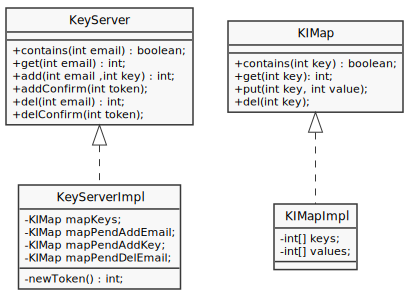
\includegraphics[width=.5\textwidth]{uml}
  \caption{UML class diagram of the Map version}
  \label{fig:umlclassdiagram}
\end{wrapfigure}
%
The second version builds upon the generalization of the previous map structure,
that are part of the first version.

\texttt{KIMap} (Key Integer Map) is an interface representing a map of int to
int. Its functionality is bound (by JML contracts) to the behavior of an
abstract map data type in theories of KeY. \texttt{KIMapImpl} is a simple
implementation based upon two int-arrays, one for the key, the other the values.
%
\texttt{KeyServer} is a version of the backend of the verifying key server using
integers as e-mail addresses and keys providing the functionality to get, add,
delete keys, and to confirm manipulative operations.
%
In contrast to the first version, an operation on an entry is not superseded by
a new manipulation request. The last confirmed operation wins. Also, a previous
requested deletion for an email-key pair $(e,k)$ can be used delete a different
pair $(e,k')$ if there was a confirmed update for the key $k$ in between the
deletion request and its confirmation.
%
Fig.~\ref{fig:umlclassdiagram} shows the classes.

\todo{Ownership approach?}

\iffalse
@startuml
hide circle
skinparam classAttributeIconSize 0
skinparam monochrome true
skinparam shadowing false

class KeyServer {
    +contains(int email) : boolean;
    +get(int email) : int;
    +add(int email ,int key) : int;
    +addConfirm(int token);
    +del(int email) : int;
    +delConfirm(int token);
}

class KeyServerImpl implements KeyServer {
    -KIMap mapKeys;
    -KIMap mapPendAddEmail;
    -KIMap mapPendAddKey;
    -KIMap mapPendDelEmail;
    -newToken() : int;
}

class KIMap {
    +contains(int key) : boolean;
    +get(int key): int;
    +put(int key, int value);
    +del(int key);

}

class KIMapImpl implements KIMap {
    -int[] keys;
    -int[] values;
}
@enduml
\fi

\subsection*{Proofed Properties}

We verified the software on a method-by-method.
%
This includes
%
This exclude the effect of multiple chained operations. \todo{MU: DId not understand}

\section{Conclusion }

We verified abstraction of the key server based on integer.
%
A next goal would be the verification of an implementation which uses String
values for the email and key. This also requires a new theory for strings and
maps in \KeY.
%
%During the verification with \KeY we found some deficiencies in \KeY.
%




\end{document}
